\documentclass{standalone}
\usepackage{tikz}
\usetikzlibrary{patterns, positioning}


\begin{document}
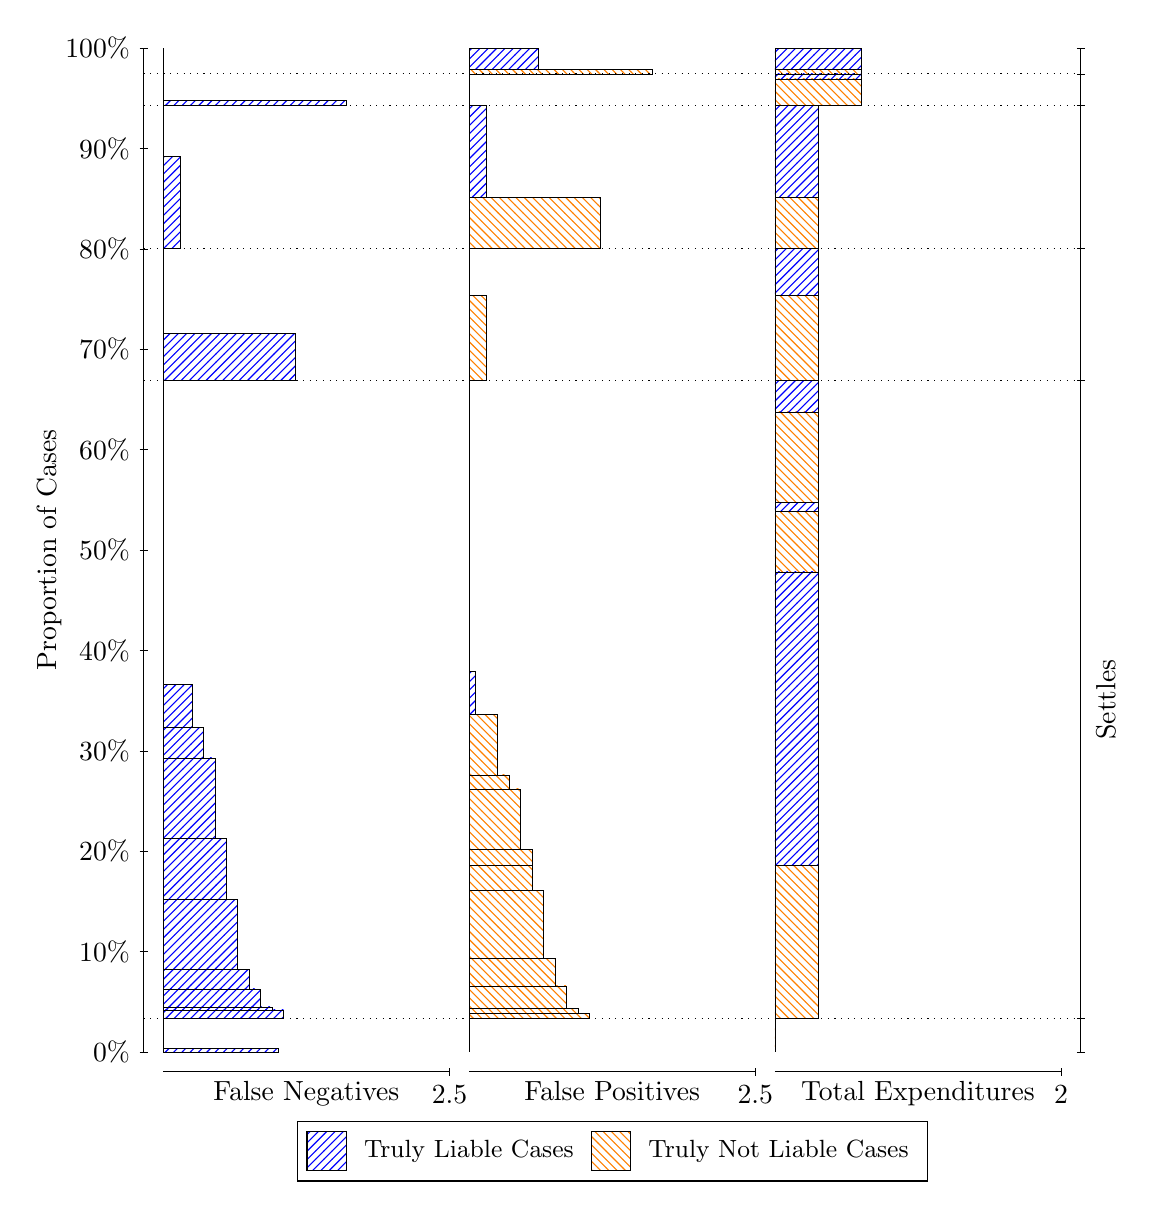
\begin{tikzpicture}
\draw[black, very thin] (1.5,1.75) -- (1.5,14.5);
\node[rotate=90, text=black, anchor=center] at (0.3, 8.125) {Proportion of Cases};
\draw[black, very thin] (1.45,1.75) -- (1.55,1.75);
\node[text=black, anchor=east] at (1.45, 1.75) {0\%};
\draw[black, very thin] (1.45,3.025) -- (1.55,3.025);
\node[text=black, anchor=east] at (1.45, 3.025) {10\%};
\draw[black, very thin] (1.45,4.3) -- (1.55,4.3);
\node[text=black, anchor=east] at (1.45, 4.3) {20\%};
\draw[black, very thin] (1.45,5.575) -- (1.55,5.575);
\node[text=black, anchor=east] at (1.45, 5.575) {30\%};
\draw[black, very thin] (1.45,6.85) -- (1.55,6.85);
\node[text=black, anchor=east] at (1.45, 6.85) {40\%};
\draw[black, very thin] (1.45,8.125) -- (1.55,8.125);
\node[text=black, anchor=east] at (1.45, 8.125) {50\%};
\draw[black, very thin] (1.45,9.4) -- (1.55,9.4);
\node[text=black, anchor=east] at (1.45, 9.4) {60\%};
\draw[black, very thin] (1.45,10.675) -- (1.55,10.675);
\node[text=black, anchor=east] at (1.45, 10.675) {70\%};
\draw[black, very thin] (1.45,11.95) -- (1.55,11.95);
\node[text=black, anchor=east] at (1.45, 11.95) {80\%};
\draw[black, very thin] (1.45,13.225) -- (1.55,13.225);
\node[text=black, anchor=east] at (1.45, 13.225) {90\%};
\draw[black, very thin] (1.45,14.5) -- (1.55,14.5);
\node[text=black, anchor=east] at (1.45, 14.5) {100\%};

\draw[black, very thin] (13.4,1.75) -- (13.4,14.5);
\draw[black, very thin] (13.35,1.75) -- (13.45,1.75);
\node[anchor=west] at (13.35, 1.75) {};
\draw[black, very thin] (13.35,2.1748) -- (13.45,2.1748);
\node[anchor=west] at (13.35, 2.1748) {};
\draw[black, very thin] (13.35,10.28) -- (13.45,10.28);
\node[anchor=west] at (13.35, 10.28) {};
\draw[black, very thin] (13.35,11.954) -- (13.45,11.954);
\node[anchor=west] at (13.35, 11.954) {};
\draw[black, very thin] (13.35,13.772) -- (13.45,13.772);
\node[anchor=west] at (13.35, 13.772) {};
\draw[black, very thin] (13.35,14.171) -- (13.45,14.171);
\node[anchor=west] at (13.35, 14.171) {};
\draw[black, very thin] (13.35,14.5) -- (13.45,14.5);
\node[anchor=west] at (13.35, 14.5) {};

\draw[black, very thin, pattern color=blue, pattern=north east lines] (1.75,1.75) rectangle (3.2033,1.7947);
\draw[black, very thin, pattern color=orange, pattern=north west lines] (1.75,1.7947) rectangle (1.75,2.1748);
\draw[black, very thin, pattern color=blue, pattern=north east lines] (1.75,2.1748) rectangle (3.276,2.2837);
\draw[black, very thin, pattern color=blue, pattern=north east lines] (1.75,2.2837) rectangle (3.1307,2.3231);
\draw[black, very thin, pattern color=blue, pattern=north east lines] (1.75,2.3231) rectangle (2.9853,2.5506);
\draw[black, very thin, pattern color=blue, pattern=north east lines] (1.75,2.5506) rectangle (2.84,2.8031);
\draw[black, very thin, pattern color=blue, pattern=north east lines] (1.75,2.8031) rectangle (2.6947,3.6921);
\draw[black, very thin, pattern color=blue, pattern=north east lines] (1.75,3.6921) rectangle (2.5493,4.4583);
\draw[black, very thin, pattern color=blue, pattern=north east lines] (1.75,4.4583) rectangle (2.404,5.4842);
\draw[black, very thin, pattern color=blue, pattern=north east lines] (1.75,5.4842) rectangle (2.2587,5.8677);
\draw[black, very thin, pattern color=blue, pattern=north east lines] (1.75,5.8677) rectangle (2.1133,6.4159);
\draw[black, very thin, pattern color=orange, pattern=north west lines] (1.75,6.4159) rectangle (1.75,10.28);
\draw[black, very thin, pattern color=blue, pattern=north east lines] (1.75,10.28) rectangle (3.4213,10.873);
\draw[black, very thin, pattern color=orange, pattern=north west lines] (1.75,10.873) rectangle (1.75,11.954);
\draw[black, very thin, pattern color=blue, pattern=north east lines] (1.75,11.954) rectangle (1.968,13.12);
\draw[black, very thin, pattern color=orange, pattern=north west lines] (1.75,13.12) rectangle (1.75,13.772);
\draw[black, very thin, pattern color=blue, pattern=north east lines] (1.75,13.772) rectangle (4.0753,13.834);
\draw[black, very thin, pattern color=orange, pattern=north west lines] (1.75,13.834) rectangle (1.75,14.171);
\draw[black, very thin, pattern color=orange, pattern=north west lines] (1.75,14.171) rectangle (1.75,14.233);
\draw[black, very thin, pattern color=blue, pattern=north east lines] (1.75,14.233) rectangle (1.75,14.5);
\draw[black, very thin, pattern color=orange, pattern=north west lines] (5.6333,1.75) rectangle (5.6333,2.1302);
\draw[black, very thin, pattern color=blue, pattern=north east lines] (5.6333,2.1302) rectangle (5.6333,2.1748);
\draw[black, very thin, pattern color=orange, pattern=north west lines] (5.6333,2.1748) rectangle (7.1593,2.239);
\draw[black, very thin, pattern color=orange, pattern=north west lines] (5.6333,2.239) rectangle (7.014,2.3065);
\draw[black, very thin, pattern color=orange, pattern=north west lines] (5.6333,2.3065) rectangle (6.8687,2.5907);
\draw[black, very thin, pattern color=orange, pattern=north west lines] (5.6333,2.5907) rectangle (6.7233,2.9432);
\draw[black, very thin, pattern color=orange, pattern=north west lines] (5.6333,2.9432) rectangle (6.578,3.8053);
\draw[black, very thin, pattern color=orange, pattern=north west lines] (5.6333,3.8053) rectangle (6.4327,4.1154);
\draw[black, very thin, pattern color=orange, pattern=north west lines] (5.6333,4.1154) rectangle (6.4327,4.3201);
\draw[black, very thin, pattern color=orange, pattern=north west lines] (5.6333,4.3201) rectangle (6.2873,5.0909);
\draw[black, very thin, pattern color=orange, pattern=north west lines] (5.6333,5.0909) rectangle (6.142,5.2684);
\draw[black, very thin, pattern color=orange, pattern=north west lines] (5.6333,5.2684) rectangle (5.9967,6.039);
\draw[black, very thin, pattern color=blue, pattern=north east lines] (5.6333,6.039) rectangle (5.706,6.5871);
\draw[black, very thin, pattern color=blue, pattern=north east lines] (5.6333,6.5871) rectangle (5.6333,10.28);
\draw[black, very thin, pattern color=orange, pattern=north west lines] (5.6333,10.28) rectangle (5.8513,11.361);
\draw[black, very thin, pattern color=blue, pattern=north east lines] (5.6333,11.361) rectangle (5.6333,11.954);
\draw[black, very thin, pattern color=orange, pattern=north west lines] (5.6333,11.954) rectangle (7.3047,12.605);
\draw[black, very thin, pattern color=blue, pattern=north east lines] (5.6333,12.605) rectangle (5.8513,13.772);
\draw[black, very thin, pattern color=orange, pattern=north west lines] (5.6333,13.772) rectangle (5.6333,14.108);
\draw[black, very thin, pattern color=blue, pattern=north east lines] (5.6333,14.108) rectangle (5.6333,14.171);
\draw[black, very thin, pattern color=orange, pattern=north west lines] (5.6333,14.171) rectangle (7.9587,14.233);
\draw[black, very thin, pattern color=blue, pattern=north east lines] (5.6333,14.233) rectangle (6.5053,14.5);
\draw[black, very thin, pattern color=orange, pattern=north west lines] (9.5167,1.75) rectangle (9.5167,2.1302);
\draw[black, very thin, pattern color=blue, pattern=north east lines] (9.5167,2.1302) rectangle (9.5167,2.1748);
\draw[black, very thin, pattern color=orange, pattern=north west lines] (9.5167,2.1748) rectangle (10.062,4.1154);
\draw[black, very thin, pattern color=blue, pattern=north east lines] (9.5167,4.1154) rectangle (10.062,7.846);
\draw[black, very thin, pattern color=orange, pattern=north west lines] (9.5167,7.846) rectangle (10.062,8.6166);
\draw[black, very thin, pattern color=blue, pattern=north east lines] (9.5167,8.6166) rectangle (10.062,8.7254);
\draw[black, very thin, pattern color=orange, pattern=north west lines] (9.5167,8.7254) rectangle (10.062,9.8784);
\draw[black, very thin, pattern color=blue, pattern=north east lines] (9.5167,9.8784) rectangle (10.062,10.28);
\draw[black, very thin, pattern color=orange, pattern=north west lines] (9.5167,10.28) rectangle (10.062,11.361);
\draw[black, very thin, pattern color=blue, pattern=north east lines] (9.5167,11.361) rectangle (10.062,11.954);
\draw[black, very thin, pattern color=orange, pattern=north west lines] (9.5167,11.954) rectangle (10.062,12.605);
\draw[black, very thin, pattern color=blue, pattern=north east lines] (9.5167,12.605) rectangle (10.062,13.772);
\draw[black, very thin, pattern color=orange, pattern=north west lines] (9.5167,13.772) rectangle (10.607,14.108);
\draw[black, very thin, pattern color=blue, pattern=north east lines] (9.5167,14.108) rectangle (10.607,14.171);
\draw[black, very thin, pattern color=orange, pattern=north west lines] (9.5167,14.171) rectangle (10.607,14.233);
\draw[black, very thin, pattern color=blue, pattern=north east lines] (9.5167,14.233) rectangle (10.607,14.5);
\draw[black, dotted] (1.5,2.1748) -- (13.4,2.1748);
\draw[black, dotted] (1.5,10.28) -- (13.4,10.28);
\draw[black, dotted] (1.5,11.954) -- (13.4,11.954);
\draw[black, dotted] (1.5,13.772) -- (13.4,13.772);
\draw[black, dotted] (1.5,14.171) -- (13.4,14.171);
\draw[black, very thin] (1.75,1.5) -- (5.3833,1.5);
\node[text=black, anchor=north] at (3.5667, 1.5) {False Negatives};
\draw[black, very thin] (5.3833,1.45) -- (5.3833,1.55);
\node[text=black, anchor=north] at (5.3833, 1.45) {2.5};

\draw[black, very thin] (5.6333,1.5) -- (9.2667,1.5);
\node[text=black, anchor=north] at (7.45, 1.5) {False Positives};
\draw[black, very thin] (9.2667,1.45) -- (9.2667,1.55);
\node[text=black, anchor=north] at (9.2667, 1.45) {2.5};

\draw[black, very thin] (9.5167,1.5) -- (13.15,1.5);
\node[text=black, anchor=north] at (11.333, 1.5) {Total Expenditures};
\draw[black, very thin] (13.15,1.45) -- (13.15,1.55);
\node[text=black, anchor=north] at (13.15, 1.45) {2};


\node[text=black, centered, rotate=90] at (13.72, 6.2274) {Settles};





\draw (7.449999999999999,1.5) node[draw=none] (baseCoordinate) {};
\begin{scope}[align=center]
        \matrix[scale=0.5, draw=black, below=0.5cm of baseCoordinate, nodes={draw}, column sep=0.1cm]{
            \node[rectangle, draw, minimum width=0.5cm, minimum height=0.5cm, pattern color=blue, pattern=north east lines] {}; &
            \node[draw=none, font=\small, text=black] (B) {Truly Liable Cases}; &
            \node[rectangle, draw, minimum width=0.5cm, minimum height=0.5cm, pattern color=orange, pattern=north west lines] {}; &
            \node[draw=none, font=\small, text=black] (B) {Truly Not Liable Cases}; \\
            };
\end{scope}

\end{tikzpicture}
\end{document}